\documentclass[12pt,a4paper,fontset=none]{ctexart}
\usepackage{ctex}
\usepackage{emptypage} 
\usepackage{fancyhdr}
\usepackage{amsmath,amsfonts,amssymb,mathtools}
\usepackage{graphicx}%插入图片用的宏包
\usepackage{mathptmx}
\usepackage{booktabs}
\usepackage[labelfont=bf]{caption}
\usepackage{indentfirst}
\usepackage{caption}
\usepackage{enumitem}
\usepackage[marginal]{footmisc}
\usepackage{subfigure}
\usepackage{fontspec}
\usepackage{geometry}
\usepackage{setspace}
\usepackage{listings}
\usepackage{xcolor}
\usepackage{float}
\usepackage{algorithm}%算法基础宏包
\usepackage{algorithmicx}%算法基础宏包,注意小写
\usepackage{algpseudocode}%算法拓展宏包,函数,Return
\newgeometry{left=3cm,top=2.5cm,bottom=2.5cm,right=3cm}
\setmainfont{Times New Roman}
\setCJKmainfont[BoldFont=SimHei,ItalicFont=KaiTi]{SimSun}
\lstset{
	backgroundcolor=\color{green!10!blue!15},
	rulesepcolor= \color{red!40!blue!100},
	breaklines=true,
	breakatwhitespace=false,
	numbers=left, 
	numberstyle= \small,
	keywordstyle= \color{blue},
	commentstyle=\color{gray}, 
	frame=shadowbox
}

\renewcommand{\baselinestretch}{1.5}

\title{\textbf{数据结构与算法第四次作业}}

\author{
\\
\Large{麻超 \quad 201300066}
\\[6pt]
{ \large \textit{南京大学人工智能学院}}\\[2pt]
}

\date{\today}
\newcommand{\supercite}[1]{\textsuperscript{\cite{#1}}}

\begin{document}

\maketitle
\setcounter{page}{1}
\section*{Problem 1}
\subsection*{a}
可以通过改进快速排序算法以得到一个k-sorted数组.具体方法为快速排序递归时当right-left<k时就取消递归.

由于快速排序的特性,每一次排序完成后,在主元左边的数总是比主元小,在主元右边的数总是比主元大.这样设置主元时,最左边的n/k个元素一定是最小的k个,在这之后这些元素不参加排序,那么接下来n/k个元素一定是次小的几个.这样递推下来,一定是符合k-sort的要求的.

在最优情况下,即每次都能平分数组时,可以得到时间复杂度为T(n)=T(n/2)+n.

其中这个递归树在最优情况下一共需要递归$\log_2 k$次,即递归树深度为$\log k$,每层需要遍历所有元素,故相乘之后时间复杂度为$O(n\log k+n)=O(n\log k)$.
\subsection*{b}
对于一个数组而言,其最小的n/k个数字是确定的,但顺序不定.即每个子数组中的数据都是确定的.然而任何基于比较的排序算法都是基于二叉树排列的,即对所有的$(k!)^{n/k}$种情况都能够做出排列,即该二叉树必须至少有这么多叶节点,所以决策树的高度至少为$2^h\geq (k!)^{n/k}$
\begin{align*}
	h\geq \frac{n}{k}\cdot lg(k!)\geq \frac{n}{k}\cdot (\frac{k\ln k-k}{\ln 2} )=\frac{n\ln k-n}{\ln 2}=\Omega(n\lg k)
\end{align*}

即至少需要$\Omega(n\lg k)$次比较.
\section*{Probelm 2}
\subsection*{a}
分为两组硬币后,依然有两个假币,一个比较重一个比较轻.当这两个不在同一边时,其重量不同,当这两个在同一边时,其重量相同.故要求的概率就是两个假币在同一边的概率.当n较大时,可以近似认为每一个硬币在前一堆和后一堆的概率都是1/2.故$P=2*1/2*1/2=1/2$.即两边重量相同的概率是1/2.
\subsection*{b}
过程1:每次将硬币分为两堆,再根据1的结论,判断两个假币在同一边或者不在同一边.如果其在同一边,则需要对两个大小为n/2的硬币堆都再次进行判断,直到找出重的和轻的硬币分别在哪一堆.当找到这两枚假币分别在哪一堆之后就可以用新的算法来分别找出这两枚硬币.

过程2:新的算法也很常见,就是将该硬币堆分为三堆(事实上当n为2的幂时无法被3整除,此时只需要尽量保证三堆的元素个数近似相同且至少有两堆元素个数相同),然后将数目相同的两堆进行比较(此时假设需要找的是轻的假币),若有一堆比较轻,则证明假币在这一堆里面,如果两堆重量相同,则证明假币在第三堆中,再次递归循环,直到找出假币所在位置,重的假币同理.

在过程一中,即找出两个假币分别在哪一堆时,有1/2的概率没有办法找出,另有1/2的概率可以找出(来自(1)),在找出之前,每次都维持着原来的问题规模不变,一旦找到,问题规模就会缩小至$n(\frac{1}{2})^k $(k为过程1的执行次数).在找出之后,每次递归可以减少至原来1/3的复杂度.由于过程1可以近似理解为服从参数p为1/2的几何分布,故执行次数的期望E(x)=2.即期望意义下需要执行两次过程1.在这种情况下,会将问题缩小至n/2的规模(两个n/4规模大小的问题).

故时间复杂度$T(n)=T(n/2)+O(1)=T(n/6)+O(1)=...=O(\log_3 n)$
\section*{Probelm 3}
\subsection*{a}
首先对数组W进行循环求和,计算出w(S),以供后续比较.

其次,利用一个时间复杂度为O(nlg n)的排序算法(可以是快速排序,归并排序等...)对数组S进行排序,并在对数组S排序时调整数组W中元素的位置,以确保二者元素可以一一对应.接下来只需要对数组S进行遍历,依次求出S对应的weight的值的和,并将其与w(S)/2进行比较,直至其可以满足所述条件.

时间复杂度:第一次计算总和的时间复杂度为O(n),排序算法的时间复杂度为O(nlg n),后面计算部分和并与之比较的时间复杂度也为O(n),故总的时间复杂度为O(nlg n).
\subsection*{b}
第一步和(a)一样首先计算所有weight的和,以便后边进行比较.首先按照Select函数寻找主元的方法找到主元,其次按照所得到的主元的值对数组S进行Partition划分,将小于主元的划分在S左边,将大于S的划分在S右边,并同时调整数组W中元素的值,使之与S可以一一对应.计算主元两边数组S中元素对应的weight的和,如果可以满足题目中对magical-mean的定义,则返回该主元.如果不满足magical-mean的定义,则再次进行递归操作,即若左边一部分weight的和大于w(S)/2,则对左边部分进行递归,直到左边刚好满足小于w(S)/2.右半部分同理.

时间复杂度:第一次计算总和时为O(n),后面进行递归操作时由学过的知识可知该递归不会改变时间复杂度,故该算法时间复杂度为O(n).
\section*{Problem 4}
\subsection*{a}
由于只有两种元素1和0,所以只需要找一个参考元素,用其他的元素与之比较即可.然而选取的这个元素不能与0或者1比较,否则其至少需要n次比较才可以完成.可以利用与后面元素的判断来确定该参考元素的值.具体操作方法为选定一个元素a[0],令a[1],a[2],...a[n-1]与之比较,若a[1]<a[0],将其放入0的一队中,若a[1]>a[0],将其放入1的一队中,若a[1]=a[0],则先等待直到能够确定a[0]的值.另外在比较过程中,如果出现了a[i]<a[0]的情况,则可以确定a[0]的值为1,否则则可以确定a[0]的值为0.在整个比较过程中,只需要比较a[0]与其他所有元素值的大小,即需要比较n-1次.
\subsection*{b}
利用桶排序的思想对其进行排序.首先建立26个桶,分别对应字母a-z.然后根据每个字符的首字母将其放入26个桶内,然后再在每一个桶内对这个桶内的字符串的第二个字母(没有第二个字母时放在最前面)排序,依次类推,最后按照桶的顺序和桶内元素的顺序将字符串放入数组内,排序即可完成.由于所有的字符串字符总和为n,故假设第一次共有k个字符,排序需要O(k)时间,后面的排序同理,总的时间复杂度为O(n).
\section*{Problem 5}
\subsection*{a}
利用数学归纳法证明结论.

奠基:当n=1时,则该根节点即为central vertex.

归纳假设:设当n=k时该结论可以成立,即当n=k时该树存在一个central vertex使得该树可以被分为三个子树,且每个子树含有的顶点树均不大于n/2.

归纳递推:如果证明当n=k+1时,无论n=k时是怎样的情况,都可以得到该结论正确,则由数学归纳法的基本思想可以得知该结论是正确的.分为以下几种情况:

1.如果当n=k时所得到的三个子树节点数都不大于n/2,则添加一个节点后,无论添加在哪个位置,它必然时这三个子树的其中一个子树的叶节点,则这三个子树的节点数同样不会超过(k+1)/2,可以得知正确.

2.如果当n=k时得到的三个子树其中一个子树节点数为n/2(T1),其他两个小于或等于n/2(T2,T3),但和不会超过n/2.当该节点添加到T2,T3时,同样满足原条件,可以证明.以下只讨论添加叶节点到T1的情况.分为以下子情况:

1).如图所示,当原来的central vertex为根节点时,可以选择将central vertex向T1移动,便可维持T1的规模不变,将T2(没有T3)的规模增加1.当k为奇数时,T2的规模是n/2-1,变化后,变为n/2.满足条件.
\begin{figure}[H]
	\centering
	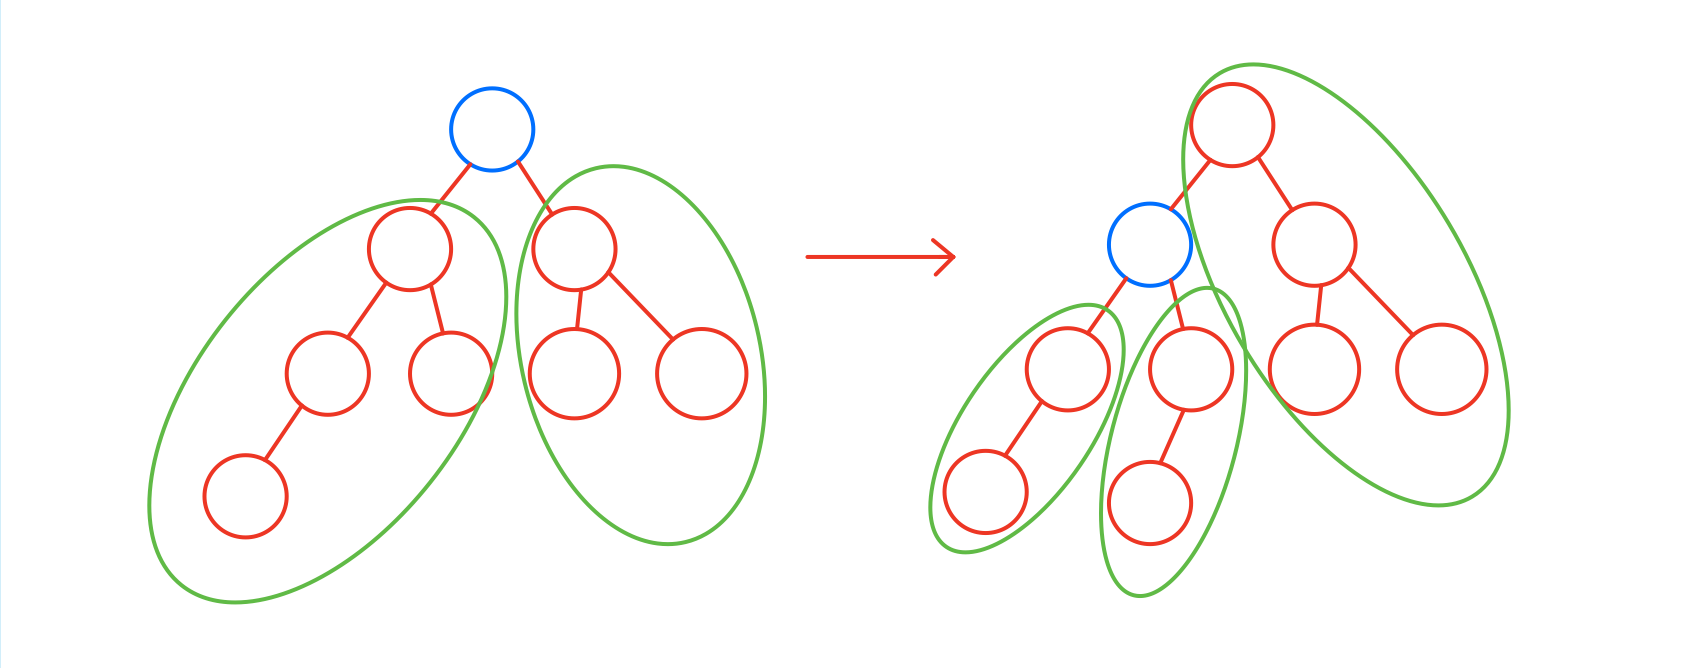
\includegraphics[width=0.7\linewidth]{题图1.png}
\end{figure}
2).如图所示,当原来的central vertex不是根节点时,可以选择将central vertex向根节点移动,可维持T1的规模,并且T1的规模保持n/2时,可以保证剩下一部分(或两部分)的规模也不会超过n/2.满足条件.
\begin{figure}[H]
	\centering
	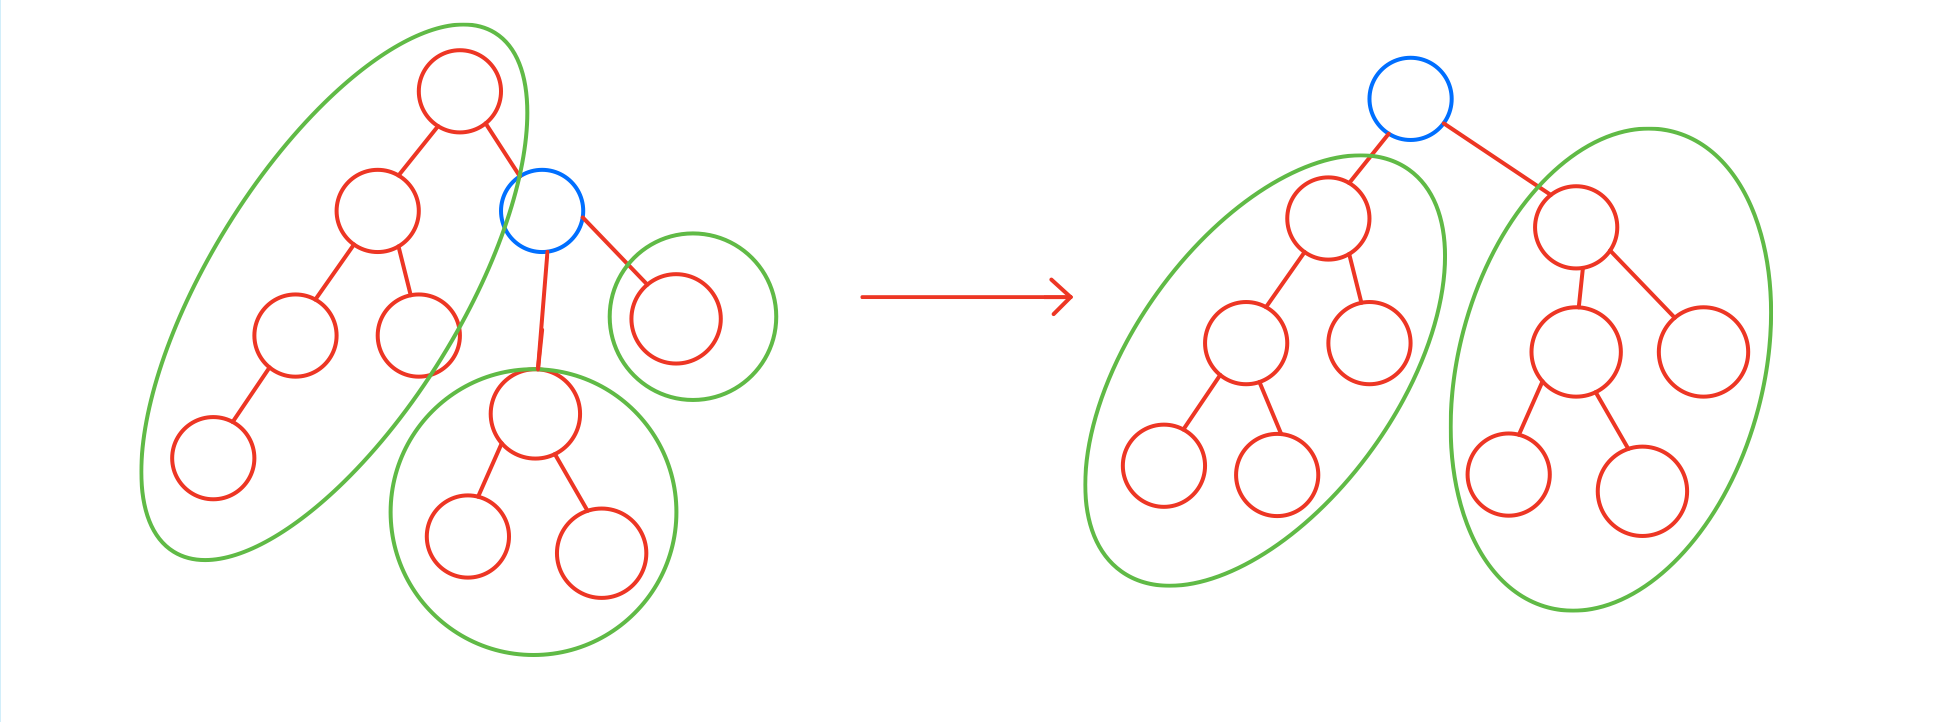
\includegraphics[width=0.7\linewidth]{题图2.png}
\end{figure}
3)central vertex不可能为叶节点.

由上述数学归纳法过程可知,对于所有的树,都至少有一个central vertex.
\subsection*{b}
通过检查每一个树或子树的节点树来判断是否为central vertex.当前指向root节点,则判断root节点的左子树和右子树所包含的顶点有多少个,若二者相等(平衡二叉树),则该root节点即为central vertex.否则,则指向包含顶点数多的该节点,将该节点的左子树所含顶点数目与右子树所含顶点数目与上一轮得到的另一个子树包含的顶点数目+1做比较,若三者中的最大值不超过n/2,则该节点即为central vertex.否则,继续移动向该节点包含顶点数多的子树的顶点.直到找到某个顶点满足central vertex的要求为止.

\section*{Problem 6}
\subsection*{a}
要找A和B的并集的第k小元素,考虑利用二分法.

首先假设k为偶数,当A,B的元素数量都大于k/2时,比较A[k/2-1](即A中第k个元素),B[k/2-1](B中第k个元素),比较的结果分为三种情况:
\begin{itemize}
	\item A[k/2-1]<B[k/2-1],此时说明A中最多有在k/2-1之前的数和B中k/2-1之前的数,共k-2个数大于A[k/2-1],即其不可能是第k小的数.此时排除A中A[0,...k/2-1]这k/2个元素.
	\item A[k/2-1]>B[k/2-1],同理,删除B[0,...k/2-1]这k/2个元素.
	\item A[k/2-1]=B[k/2-1].此时即找到了第k小的元素,返回A[k/2-1]或B[k/2-1]即可.
\end{itemize}
这之后,如果没有找到,则再次进行递归,更新k的值,即令k=k-k/2.继续取A[k/2-1]和B[k/2-1]进行比较.(注意此时有一个数组中删除了k/2个元素.)则反复递归,利用二分查找法找到第k小的值.

如果A和B中有一个数组的剩余值已不足k/2,则取该数组的全部元素,不足的部分由B来补齐.在这种情况下,k后来的取值应该以排除的个数来决定,而不是直接减去k/2.另外,当k=1时,可以直接输出A和B当中的最小值.当某一个数组为空时(已经被全部排除),可以直接输出另一个数组第k小的值.

伪代码如下:
\begin{algorithm}
	\renewcommand{\algorithmicensure}{\textbf{Output:}}
	\renewcommand{\algorithmicrequire}{\textbf{Input:}}
	\caption{find the $k_{th}$ smallest number in A$\cup$B }
	\label{alg1}
	\begin{algorithmic}
		\Require $A[],B[],k,A.length=m,B.length=n$
		\Function{GetKthElement}{$A[],B[],k$}
		\State $index1,index2\gets 0$
		\While {True}
		\If  {index1==m}
		\State \Return $B[index2+k-1]$
		\EndIf
		\If{index2==n}
		\State \Return $A[index1+k-1]$
		\EndIf
		\If{k==1}
		\State \Return $min(A[index1],B[index2])$
		\EndIf
		\State $newIndex1\gets min(index1 + k/2 - 1, m - 1)$
		\State $newIndex2\gets min(index2+ k/2-1,n-1)$
		\If {$A[newIndex1]\leq B[newIndex2]$}
		\State $k\gets k-newIndex1-index1+1$
		\State $index1=newIndex1+1$
		\Else
		\State $k \gets k-newIndex2-index2+1$
		\State $index2=newIndex2+1$
		\EndIf
		\EndWhile
		\EndFunction
		\Ensure $GetKthElement(A,B,k)$
	\end{algorithmic}
\end{algorithm}
时间复杂度:m,n为数组A和B的长度,由于每次查找都可以缩小一半范围,所以时间复杂度为$O(\log (m+n))$
\subsection*{b}
要想在O(1)空间内实现遍历树中的所有元素,则需要考虑在输出某个左孩子,右孩子都为空的节点后继续输出下一个节点,在中序遍历中,即代表了其某个祖先节点.因此考虑在遍历该孩子之后,指向下一个要遍历的元素(其祖先节点).得到以下方法:

在该方法中,首先给定一个树的root节点,然后寻找该root节点的左子树最右边的节点(即中序遍历时其前一个元素),该节点必定是没有右孩子的,故令其右指针指向root节点,然后指针指向root节点的左孩子,继续遍历,往此反复,可以得到以下步骤:

1.如果当前节点的左孩子为空,则输出当前节点并将其右孩子作为当前节点(指针指向下一个节点).

2.如果当前节点的左孩子不为空,在当前节点的左子树中找到当前节点在中序遍历下的前驱节点(即最"右"的节点).

a)如果前驱节点的右孩子为空,将它的右孩子设置为当前节点.令当前节点的左孩子成为当前节点.

b)如果前驱节点的右孩子为当前节点,将它的右孩子重新设为NULL(恢复树的形状)并输出当前节点.令当前节点的右孩子成为当前节点.

3.重复以上1及2步骤直到当前节点为空,即该树的所有元素都被输出了.

伪代码如下:
\begin{algorithm}
	\caption{print the tree}
	\label{alg2}
	\begin{algorithmic}
		\Require  $Tree A,node *cur=root,*prev=NULL$
		\While {cur!= NULL}
		\If {cur.left== NULL}\Comment{1.}
		\State $Print(cur.value)$
		\State $cur\gets cur.right$
		\Else
		\State $prev\gets cur.left$
		\While {$prev.left\neq NULL\&\&prev.right\neq cur$}
		\State $prev\gets prev.right$
		\EndWhile
		\If {prev.right==NULL}\Comment{2.a}
		\State $prev.right\gets cur$
		\State $cur\gets cur.left$
		\Else \Comment{2.b}
		\State $prev.right\gets NULL$
		\State $Print(cur.value)$
		\State $cur\gets cur.right$
		\EndIf
		\EndIf
		\EndWhile
	\end{algorithmic}
\end{algorithm}
复杂度分析:

由于在该过程中只使用了两个辅助指针,故空间复杂度为O(1).

每个树有n个结点,故有n-1条边,在整个遍历过程中每一条边最多只被走两次,一次是为了定位到某个节点,另一次是寻找某个节点的前驱节点,故其时间复杂度为O(n).
\end{document}